\scanpage{61}
Partant des MD-graphes ``élémentaires'' correspondants, je voudrais expliciter dans les quatre cas la structure \inserted{de spécialisation entre} des strates des $\widehat M_{g,\nu}$ et $\widehat M^!_{g,\nu}$.

8) \uline{Structure de spécialisation des strates en dim modulaire $\leq2$.}

$1^\circ)$ \uline{Cas de} $\widehat M^!_{0,4}$ \uline{et} $\widehat M_{0,4}$

Commençons par $\widehat M^!_{0,4}$.
\[
(76)\quad\left\{\diagram{\begin{array}{c|c}
\text{Codim }0&\text{Codim }1\\\hline
\figure{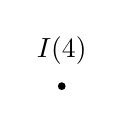
\begin{tikzpicture}[baseline=-2pt]\fill (0,0) circle (1.4pt);\node[above] at (0,.15) {$I(4)$};\end{tikzpicture}}\quad\xrightarrow{3}&
\figure{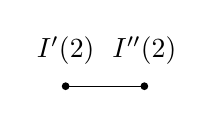
\begin{tikzpicture}[baseline=-2pt]\draw (0,0)--(1,0);\fill (0,0) circle (1.4pt);\fill (1,0) circle (1.4pt);\node[above] at (0,.15) {$I'(2)$};\node[above] at (1,.15) {$I''(2)$};\end{tikzpicture}}
\end{array}}\right.
\]
Le diagramme signifie que l'ens. marqué $I$ de cardinal $4$, \inserted{\unsure{se partageant}} suivant l'une quelc. des trois partitions de $I$ en $I'$ et $I''$ de cardinal $2$ chacun, donne $3$ spécialisations différentes de la strate maxima --- cela correspond bien sûr aux trois pts à l'infini de $U_{0,3}$

on aura
\[
(77)\qquad \widehat M^!_{0,4}\simeq\mathbf P^1_{\mathbf Z},\quad M^!_{0,4}\simeq(U_{0,3})_{\mathbf Z}=\mathbf P^1_{\mathbf Z}\smallsetminus\{0,1,\infty\}
\]
Pour bien faire, il faudrait aussi expliciter
\margin{60}
